
\documentclass[11pt]{article}
\usepackage[utf8]{inputenc}
\usepackage[T1]{fontenc}
\usepackage{blindtext}
\usepackage{amssymb}
\usepackage{amsmath}
\usepackage{float}
\usepackage[table,xcdraw]{xcolor}
\usepackage{ulem}
\usepackage{blindtext}
\usepackage[english]{babel}
\usepackage{color}
\usepackage[papersize={210mm,297mm},top=2.5cm, bottom=2.5cm, left=2cm , right=2cm]{geometry}
\usepackage{amsthm}
\usepackage{mathrsfs}
\usepackage{enumitem}
\usepackage{color}
\usepackage{xcolor}
\usepackage{graphicx}
%\usepackage{natbib} 
\usepackage{titlesec}
\usepackage{subfig}
\usepackage{amsmath}
\usepackage{mathtools}
\usepackage{lipsum}
\usepackage{adjustbox}
\usepackage{setspace}
\usepackage[colorlinks=true, linkcolor=blue]{hyperref}
\usepackage{siunitx}
\usepackage{tikz}
\usetikzlibrary{snakes}
\usepackage{wrapfig}
\definecolor{light-gray}{gray}{0.95}
\usepackage{tcolorbox}
\usepackage{fancyhdr}
\usepackage{xcolor}
\usepackage{lastpage}
\usepackage{changepage}
\usepackage{titlesec}
\usepackage{titling}
\usepackage{blindtext}
\usepackage{setspace}
\usepackage{blindtext}
\usepackage{multicol}
\usepackage[style=verbose]{biblatex}
\usepackage{caption}
\usepackage[toc,page]{appendix}
\usepackage{listings}



\begin{document}

\pagestyle{fancy}
\lhead{\textit{\textbf{Computational Motor Control, Spring 2019} \\
    Python exercise, Lab 5 and 6}} \rhead{Students : Hedi Fendri , Sascha Frey, Elias Gajo}

\section*{Student names: Hedi Fendri, Sascha Frey, Elias Gajo}
\section*{Introduction}
In this practical, we investigate the behaviour of muscles, neurons and their interactions in different conditions by conducting experiments on numerical models. 


\section*{Exercise 1 : Hill muscle model}
\label{sec:question-2}

\subsection*{Muscle Force-Length Relationship}
\label{sec:muscle-force-length}

\subsection*{1.a For a given stimulation, explore the relationship
  between active and passive muscle forces and the length of the
  contractile element.  Plot the force-length relationship curve.
  Discuss the different regions in the plot. Use the
  \fileref{isometric\_muscle\_system.py::IsometricMuscleSystem} instance
  to setup your experiment in \fileref{exercise1.py}}
  
In order to explore the relationship between the different forces and the length of the contractile element we conduct a series of experiments with a numerical implementation of the Hill muscle model. In each numerical experiment we give a stimulation to the muscle for a given tendon-to-tendon length and observe the reaction. We are particularly interested in the remaining forces in the muscle at the end of the experiment. A single integration experiment is given in Figure \ref{fig:experiment}

\begin{figure}[!h]
\centering
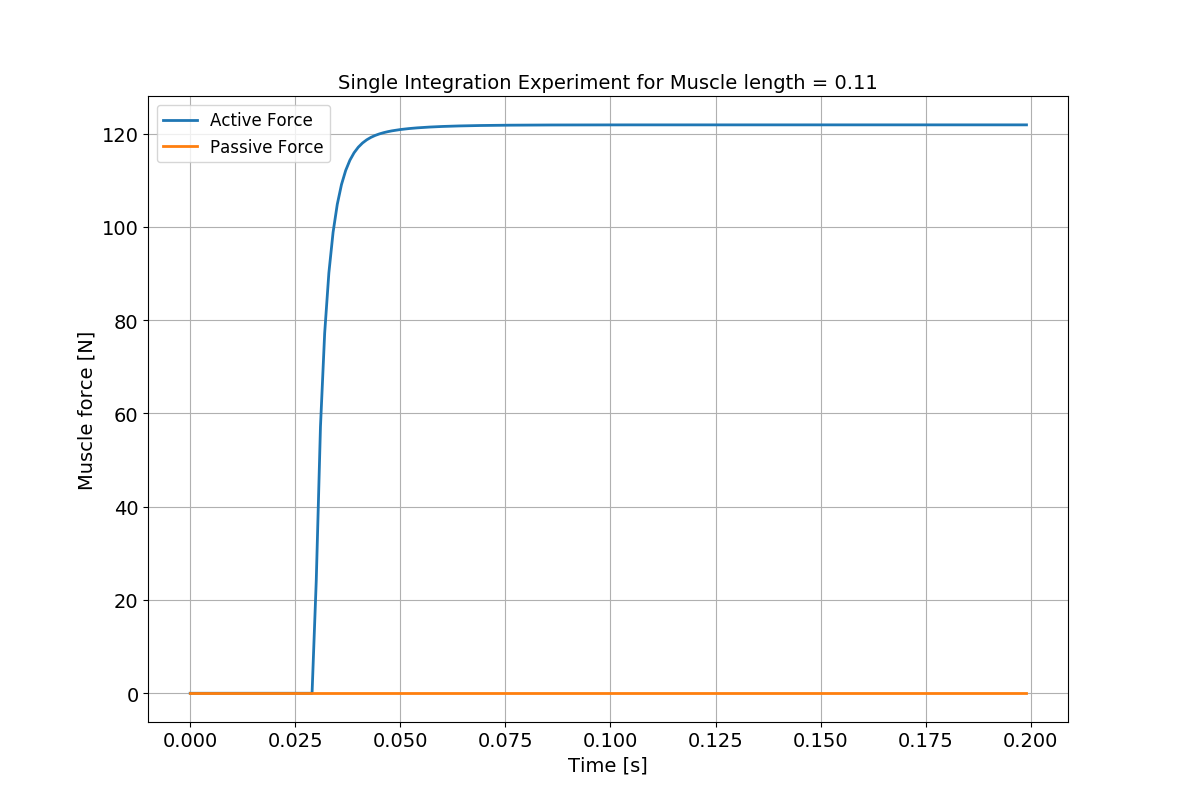
\includegraphics[width=0.9\textwidth]{Week_1/single_int.png}
\caption{Passive and Active Forces during a stimulation, only the final, resting, forces are considered.}
\label{fig:experiment}
\end{figure}


For each experiment we change the muscle length (I), this has a direct impact on the final length of the contractile element and is the only way one is able to influence this from outside in the event of a real experiment. We measure the Final Forces: Active Force, Passive Force and Total Force and plot them against the final contractile element length. The result is given in Figure \ref{fig:baseexp}. 

\begin{figure}[!h]
\centering
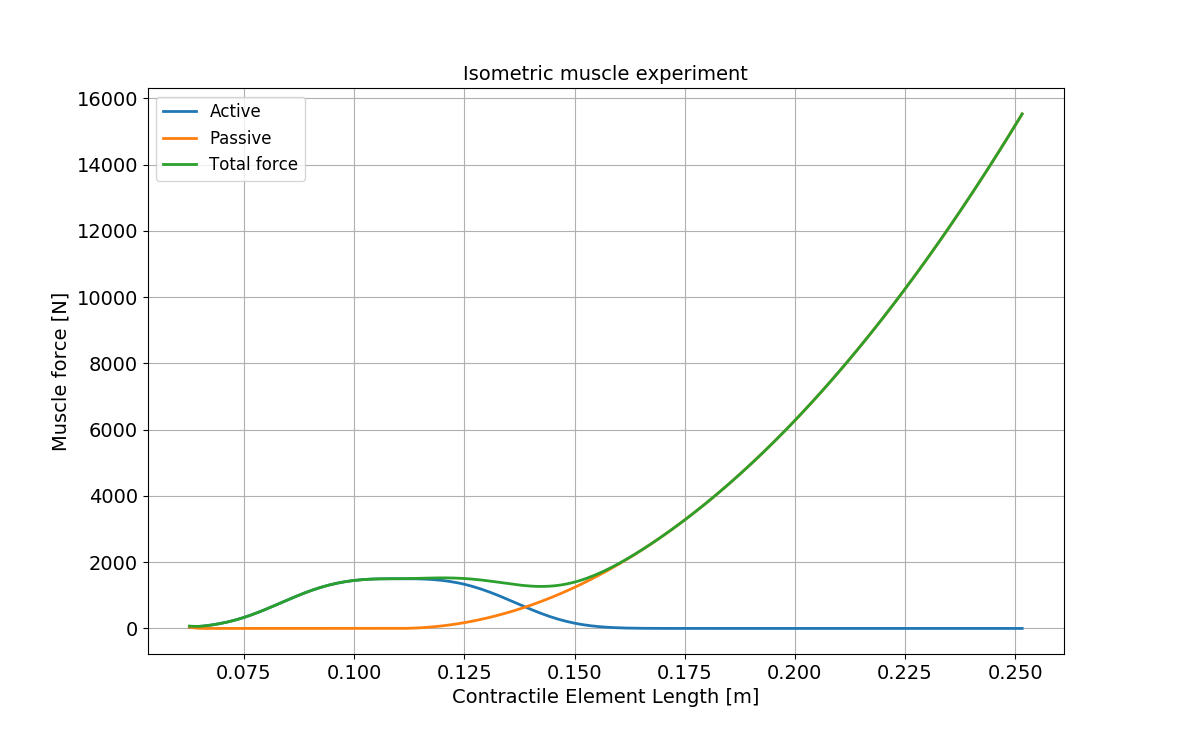
\includegraphics[width=0.9\textwidth]{Week_1/base_exp.png}

\caption{Active, Passive and Total force at rest as a function of contractile element length.}
\label{fig:baseexp}
\end{figure}

We firstly comment the active force which has a clear region of operation and a maximum. This maximum coincides with the value \(L_{opt}\) which is a parameter of the muscle. This is the length of the contractile element where the thick myosin filaments and the thin actin filaments overlap in an ideal way. This overlap is the driving factor of the active force. When there is no more overlap between the filaments then there is no more active force.

The passive force on the other hand is not limited in size and starts to grow when the muscle is significantly stretched. This can, as the Hill model suggests, simply be explained using a spring analogy, the more the muscle is extended the higher the counteracting force will be. Evidently in this numerical simulation and model there is no limit to the force that can be produced, in reality the tendons will rip when passing a maximum force. 
\newpage 
\subsection*{1.b In (1.a), you explored the muscle force-length
  relationship for a given stimulation. What happens to the
  relationship when the stimulation is varied between [0 - 1]? Support
  your response with one plot showing the different force-length
  relationship curves.}
We re-do the series of experiments done in Excercise 1.a, with different values of stimulation. The chosen values for stimulation are: [0,0.2,0.4,0.6,0.8,1]

\begin{figure}[!h]
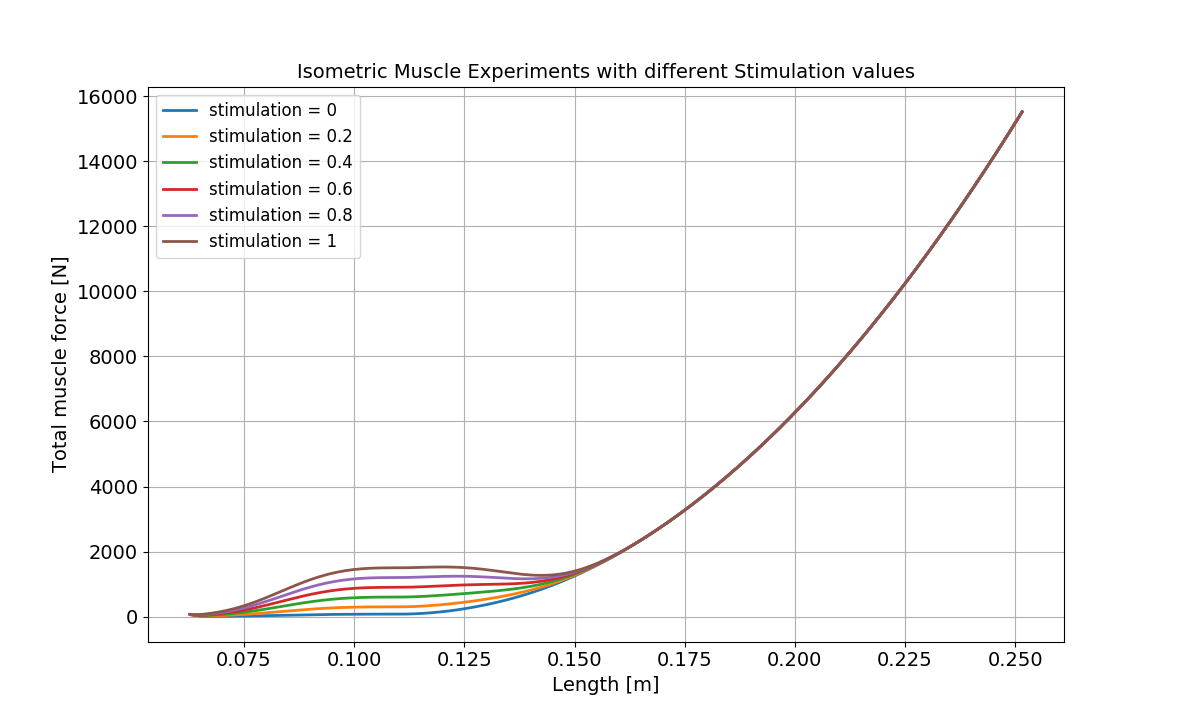
\includegraphics[width=\textwidth]{Week_1/diff_stim.png}
\centering
\caption{Total force as a function of the contractile element length for different stimulation values.}
\label{fig:stims}
\end{figure}

\begin{flushleft} Plotting the total force as a function of the contractile element length (\ref{fig:stims}), we observe that the passive component (for a length greater than 0.14) is identical for all stimulations. This leads us to conclude that the stimulation only has an affect on the active force. Furthermore, we conclude that increasing the stimulation increases the active force, if there is no stimulation at all then only the passive force is present. 
\end{flushleft}

\subsection*{1.c Describe how the fiber length ($l_{opt}$) influences
  the force-length curve.  (Compare a muscle comprised of short muscle
  fibers to a muscle comprised on long muscle fibers.). To change the
  parameter you can use
  \fileref{system\_parameters.py::MuscleParameters} before
  instantiating the muscle. No more than two plots are required. }
  
In order to understand the effect of the fiber length we have to make some changes to the model. The relevant parameter is the length \(L_{opt}\), we run a series of experiments for different fiber lengths by varying this parameter. The chosen lengths were 7cm, 11cm and 16cm respectively. The results are shown in Figure \ref{fig:lopt}.

\begin{figure}[!h]

\centering
\minipage{0.49\textwidth}
\includegraphics[width=1.25\textwidth]{Week_1/lopt_007.png}
\endminipage\hfill
\minipage{0.49\textwidth}
\vspace{0.5cm}
\includegraphics[width=1.2\textwidth]{Week_1/lopt_011.png}
\label{fig:simul_dyn_passive}
\endminipage\hfill 
\end{figure}

\begin{figure}[!h]
\centering
\includegraphics[width=0.7\textwidth]{Week_1/lopt_016.png}
\caption{Forces as a function of contractile element length for different fiber lengths.}
\label{fig:lopt}
\end{figure}

\newpage
We can conclude that the maximum active force will always be present at the optimal length, furthermore the size of this active force is unaffected by the parameter. Longer fiber lengths do not change the maximum active force, in the experiments shown the active . The fiber lengths do, however, have a strong effect on the passive force, which essentially comes into effect much faster for smaller fiber lengths. Likely this is because an identical length increase is proportionally much bigger for a small rather than a large fiber length. In the results on Figure \ref{fig:lopt}
we can see that for a contractile element length of 0.2m the passive force is 30'000 Newtons, 6'000 Newtons and 500 Newtons respectively. 


\newpage
\subsection*{Muscle Velocity-Tension Relationship}



\subsection*{1.d For a stimulation of 1.0 and starting at optimal
  muscle length, explore the relationship between contractile element
  velocity and external load. Plot the Velocity-Tension relationship
  curve. Include shortening and lengthening regions. Use the
  \fileref{isotonic\_muscle\_system.py::IsotonicMuscleSystem} instance
  to setup your experiment in \fileref{exercise1.py}}

We proceed in a similar manner as we did in analyzing the isometric situation. We run the same experiment a number of times, changing the external load. The solution to the differential equation for a single load can be observed in Figure \ref{fig:single_vel}. This image shows experiments either side of the limit condition which we will comment later. 

\begin{figure}[!h]
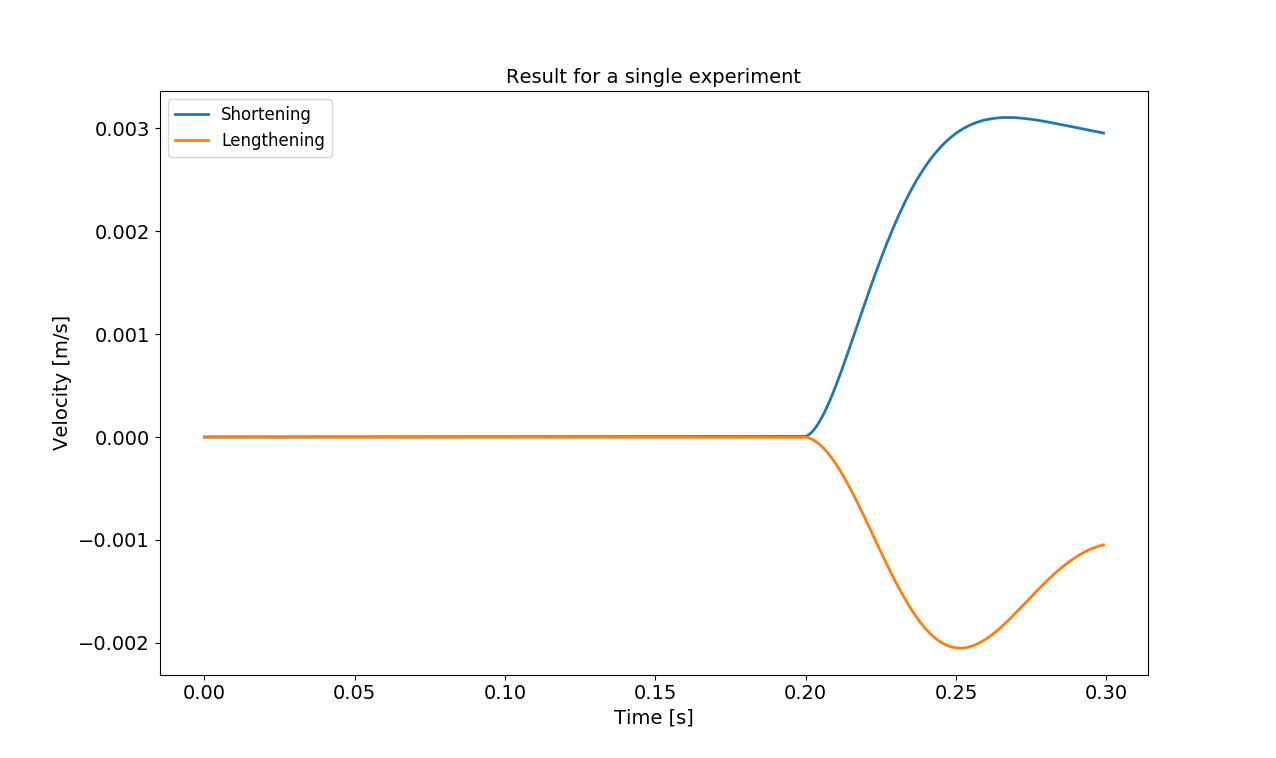
\includegraphics[width=\textwidth]{Week_1/single_int_vel.png}
\centering
\caption{Velocity as a function of time for two separate experiments either side of the limit condition. Positive velocity indicates shortening.}
\label{fig:single_vel}
\end{figure}
\newpage 
What we are most interested in is the maximum velocity during an experiment. This velocity is positive if the muscle is being shortened, i.e. the force exerted by the muscle is bigger than the attached load. If this is not the case, the velocity is negative and the muscle is lengthened. We plot on Figure \ref{fig:force_vel} the maximum velocity for a given external load in blue. We see the expected behaviour, the maximum velocity is lower for a larger load. Once passed the maximum force the muscle can exert (this is given as a parameter, in this case 1500N) the muscle is automatically lengthened. The blue curve in this case does not show the force exerted by the muscle, simply the load attached. As we were curious to replicate the theory observed in lectures shown in Figure \ref{fig:theory} we also plotted the maximum exerted active force, this allows us to observe the expected plateau in the event that the external load is larger than the maximum muscle force. 

\begin{figure}[!h]
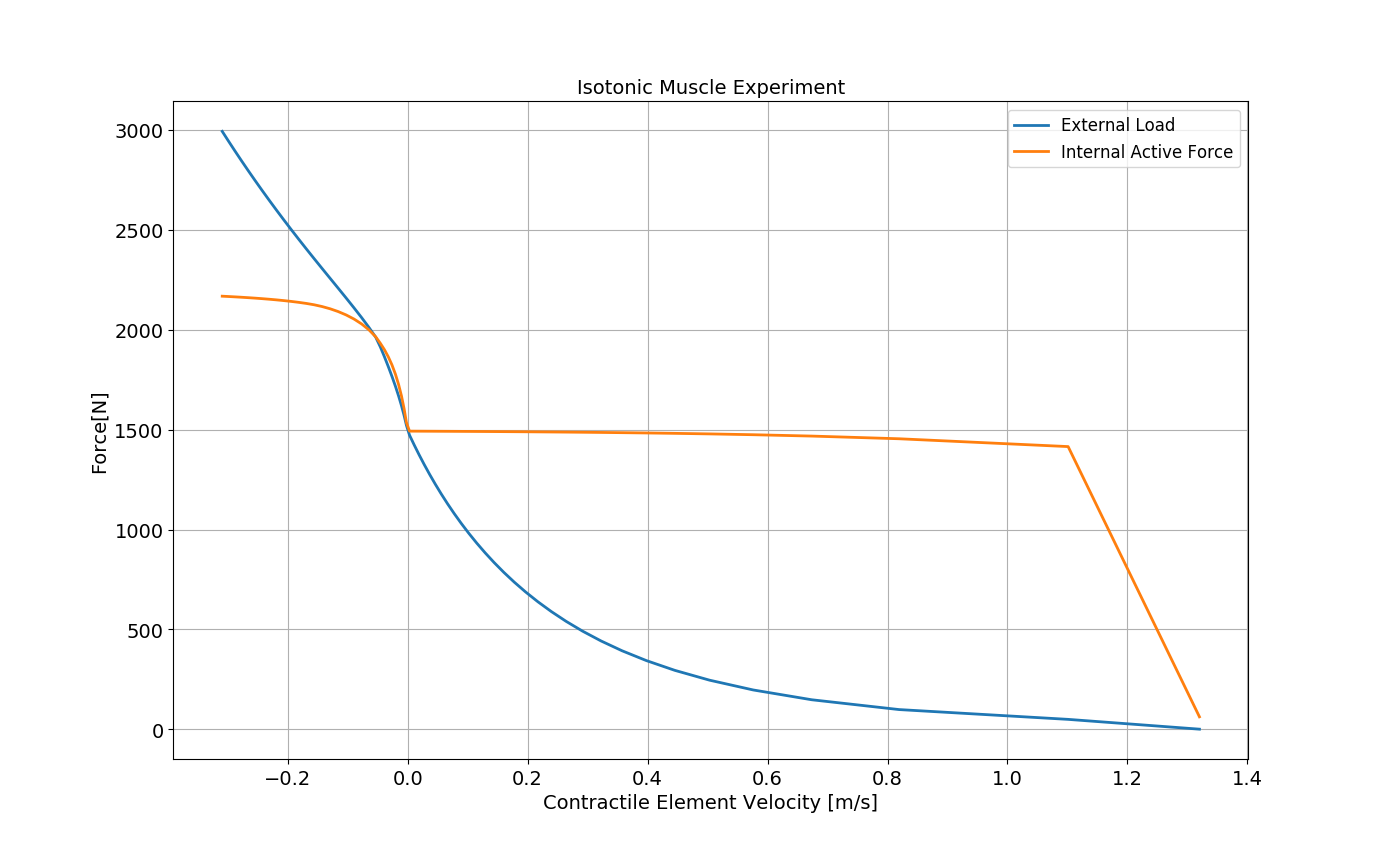
\includegraphics[width=0.8\textwidth]{Week_1/Force_velocity.png}
\centering
\caption{Maximum velocity and maximum active force for different externally applied forces.}
\label{fig:force_vel}
\end{figure}

\begin{figure}[!h]
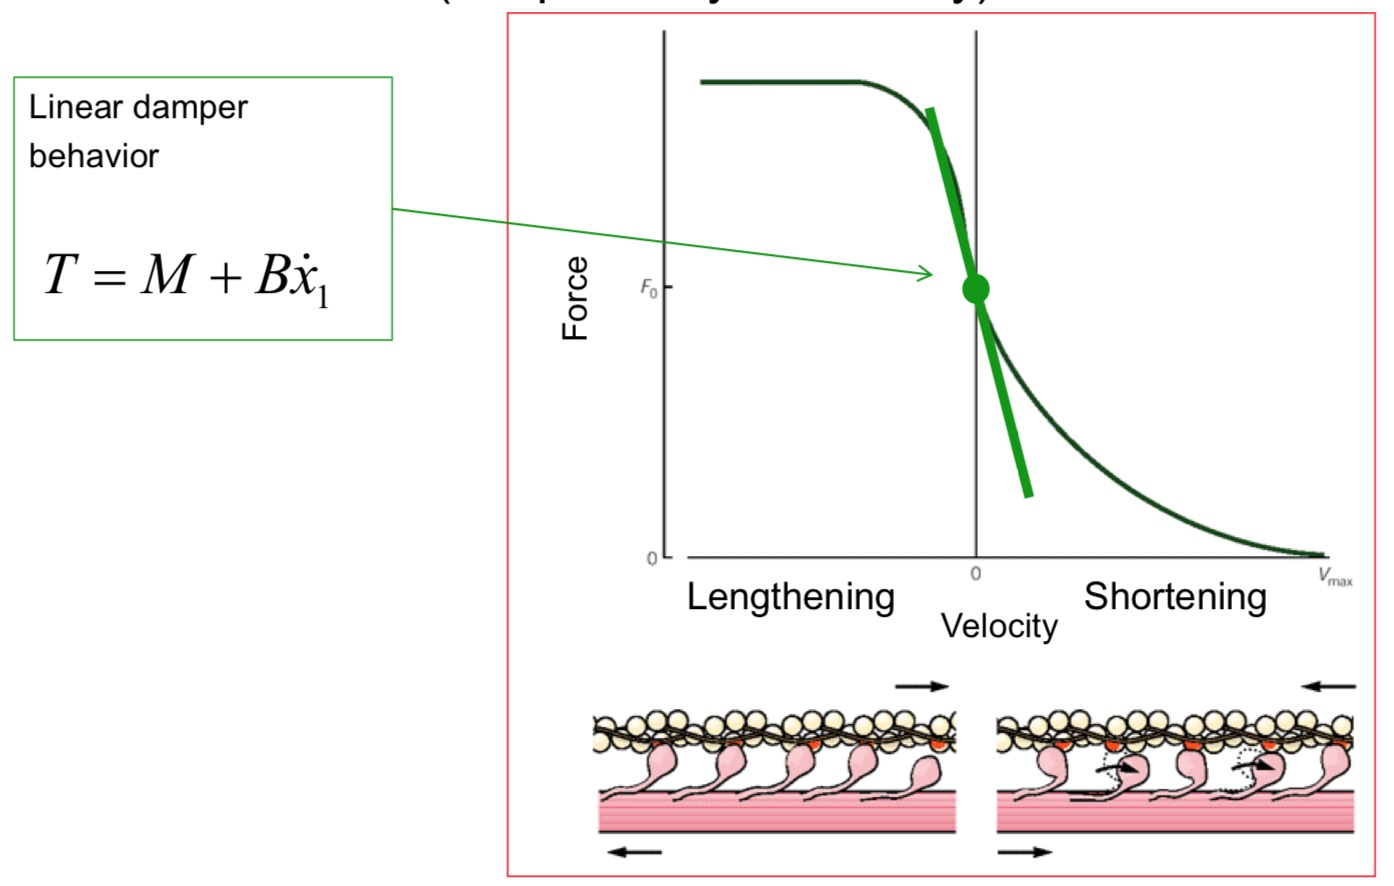
\includegraphics[width=0.8\textwidth]{Week_1/theory.jpeg}
\centering
\caption{Theoretically expected behaviour.}
\label{fig:theory}
\end{figure}


\subsection*{1.e For the muscle force-velocity relationship, why is
  the lengthening force greater than the force output during
  shortening? No plots necessary}

This behaviour is due to the damper included in the Hill Model. In the event of contracting, the damper exerts force in the direction of the contractile element. At the limit case where the contractile element force is equal to the external load, there is no velocity and therefore no damping. If the muscle is being extended then the damping element of the model still exerts force in the opposite direction of movement, only it is now in the same direction as the contractile element. Thus the total active force is larger than that exerted by the contractile element (1500 N). 

\subsection*{1.f What happens to the force-velocity relationship
  when the stimulation is varied between [0 - 1]? Support your
  response with one plot showing the different force-velocity
  relationship curves.  }
  
When varying stimulation we observe a number of differences on Figure \ref{fig:stim_var}. The key change is the maximum force which decreases linearly with stimulation, this makes sense as this force is only due to the contractile element. If this is stimulated less, the force output will be lower. 


\begin{figure}[!h]
\centering
\includegraphics[width=1\textwidth]{varrying_simulation_.png}

\caption{Varying Stimulation, both the load-velocity and force-velocity curves are shown for different stimulation values.}
\label{fig:stim_var}
\end{figure}
\newpage
\section*{Exercise 2 : Pendulum model with Muscles}
\label{sec:question-1}

\label{sec:questions}
\subsection*{2a. For a given set of attachment points, compute and
  plot the muscle length and moment arm as a function of $\theta$
  between $[-\pi/4, \pi/4]$ using equations in \corr{eqn:\ref{eq:2}}
  and discuss how it influences the pendulum resting position and the
  torques muscles can apply at different joint angles. You are free to implement
this code by yourself as it does not have any other dependencies.}
\label{sec:2a}

We firstly investigate the moment arm (h) and the muscle length (L) for the default attachment points: \(a_1=-17,17\) and \(a_2=-17\). These attachments are symmetric. We simply calculate the resulting values according to the given equation and plot accordingly. Figure \ref{fig:att1} shows the resulting length and moment arm for this first attachment configuration. We observe that the two muscles are of equal length, and have equal moment arm for an angle of 0, that is when the pendulum is vertical. This will be the case for any symmetric attachment. 

\begin{figure}[!h]

\centering
\minipage{0.49\textwidth}
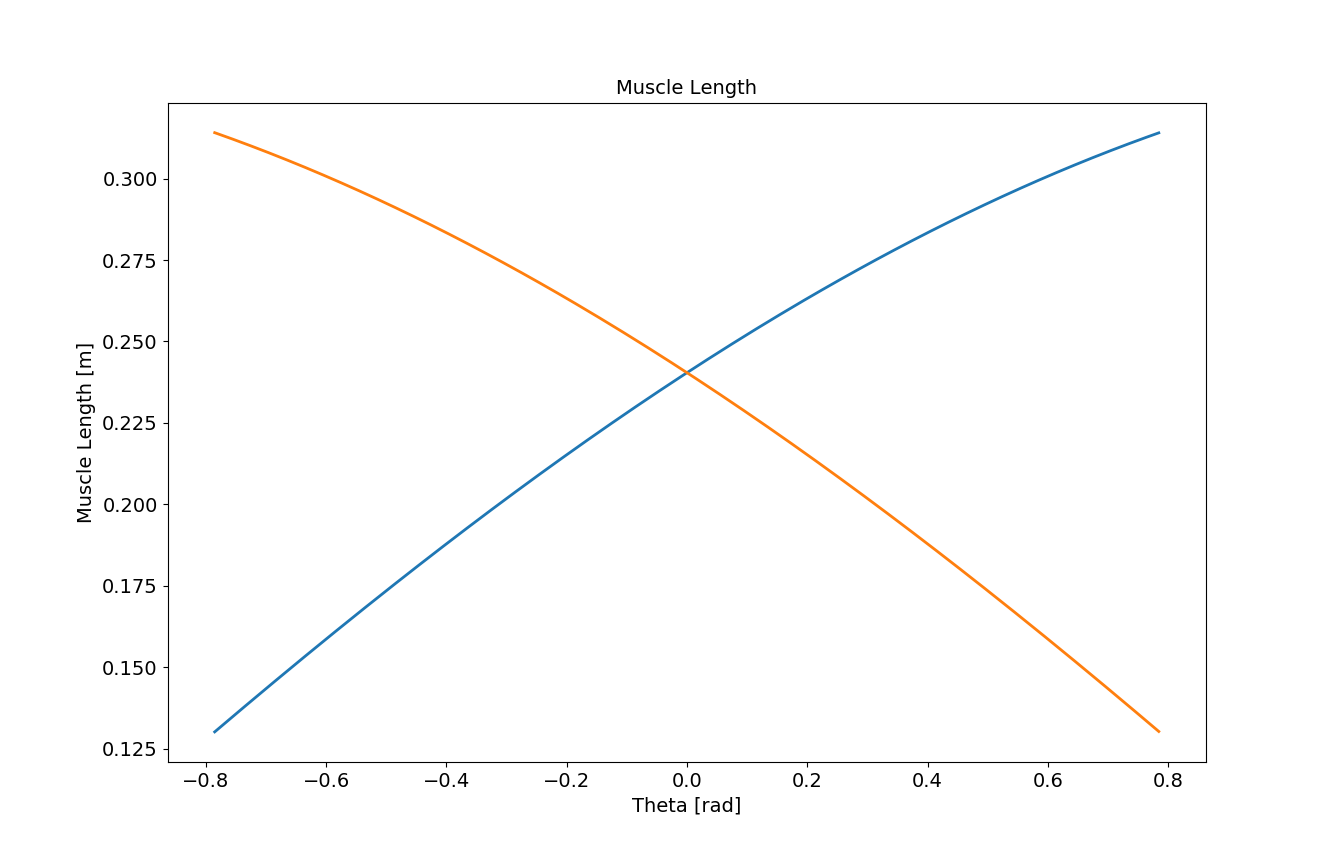
\includegraphics[width=1.1\textwidth]{Week_1/lengththeta1.png}
\endminipage\hfill
\minipage{0.49\textwidth}
\vspace{0.5cm}
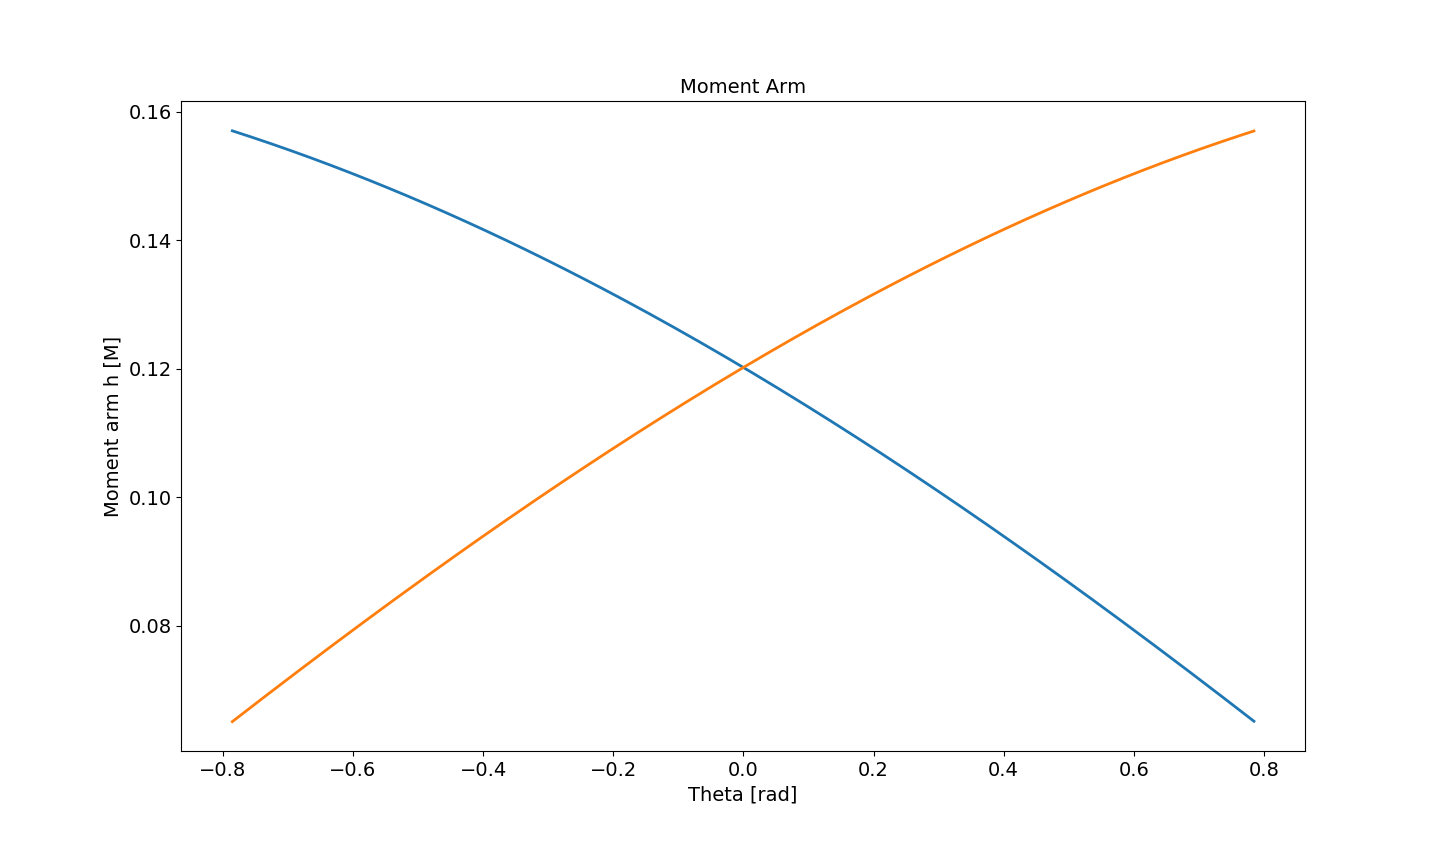
\includegraphics[width=1.2\textwidth]{Week_1/htheta1.png}


\endminipage

\caption{Muscle Length and moment arm for both muscles as a function of Theta (left muscle in blue, right muscle in red)}
\label{fig:att1}
\end{figure}


If we consider an attachment that is not symmetric: \(a_1=-10,17\) and \(a_2=-17\) then we obtain slightly different results. Notably, on Figure \ref{fig:att2} we see that the moment arm and muscle length are equal for the two muscles at different values of theta. 

\begin{figure}[!h]

\centering
\minipage{0.49\textwidth}
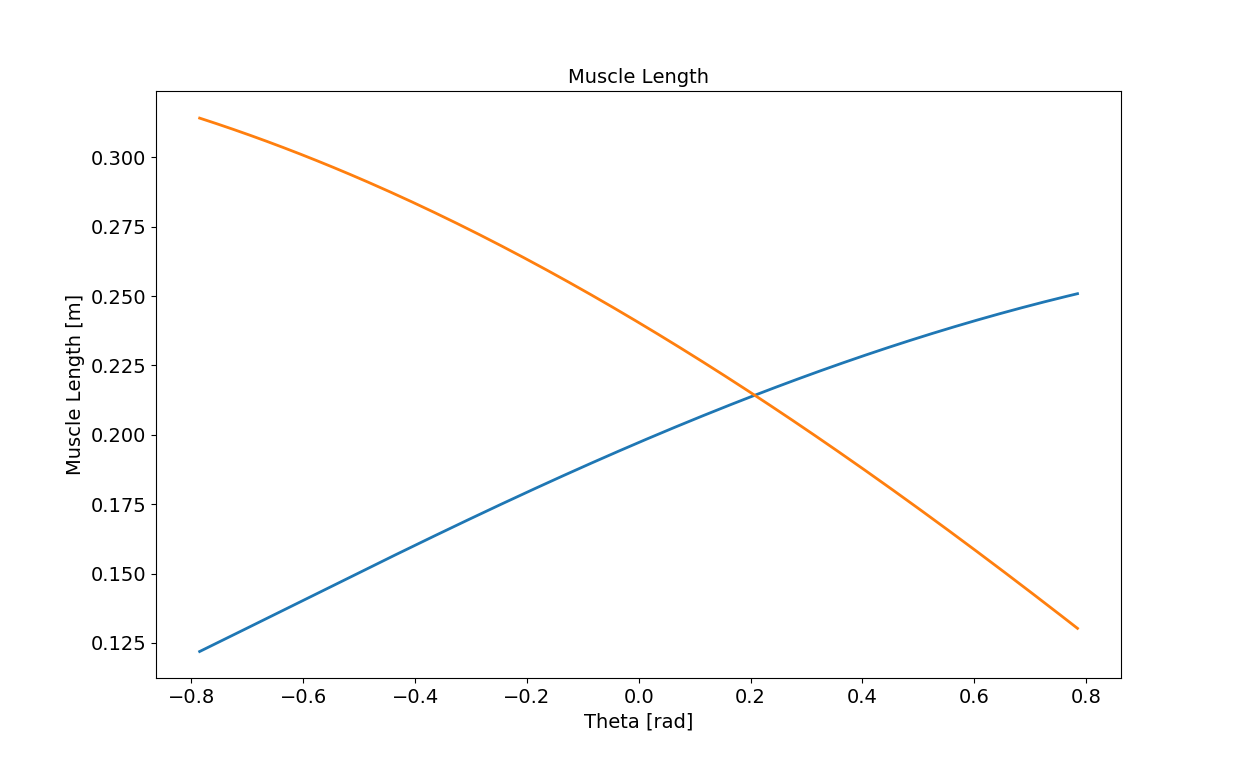
\includegraphics[width=1.1\textwidth]{Week_1/lengththeta2.png}
\endminipage\hfill
\minipage{0.49\textwidth}
\vspace{0.5cm}
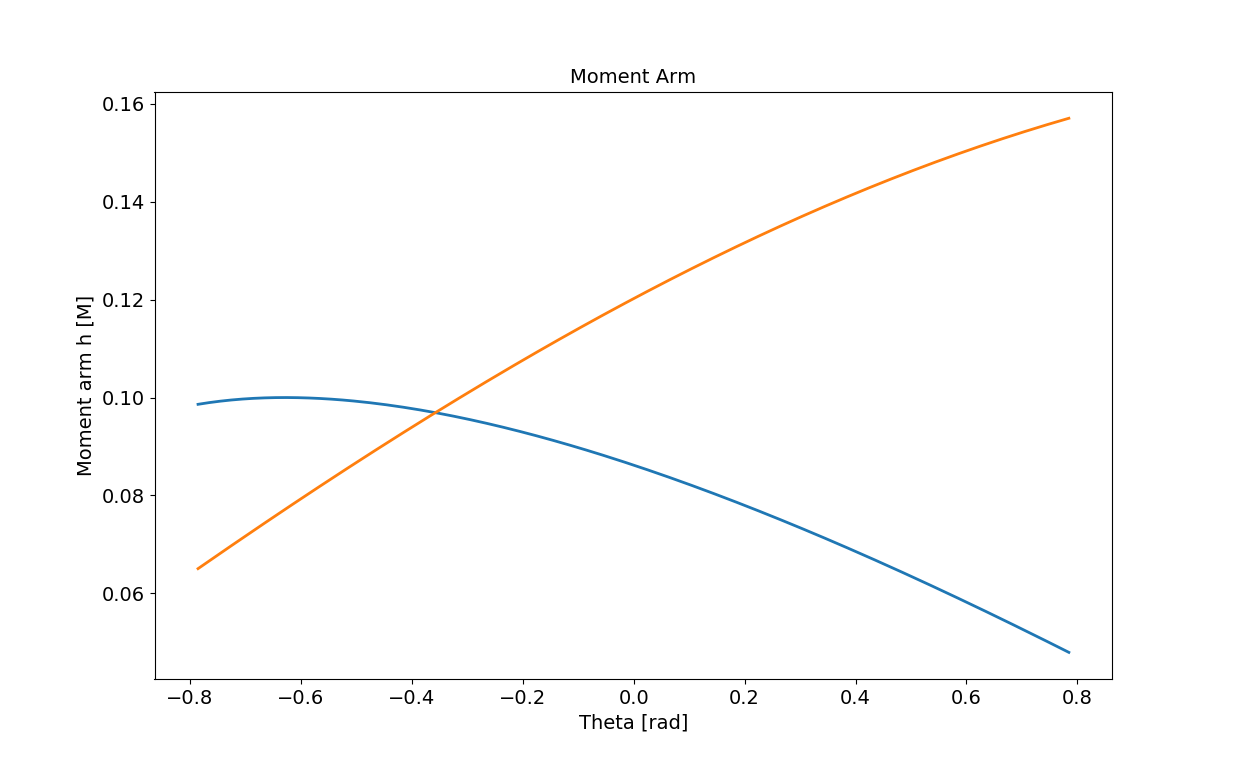
\includegraphics[width=1.1\textwidth]{Week_1/htheta2.png} 
\endminipage
\caption{Muscle Length and moment arm for both muscles as a function of Theta, for the second attachment configuration. (left muscle in blue, right muscle in red)}
\label{fig:att2}
\end{figure}

When making the assumption that the force is constant for any muscle length (in opposition to the results in Exercise 1) then we can directly observe the equilibrium position of the pendulum, depending on the attachment points of the muscles. Because \(\tau=F*h\) we know that the torque is related directly to the moment arm, the equilibrium position is therefore where the torque of the two muscles is equal. 


\subsection*{2b. Using simple activation wave forms (example : sine or
  square waves) applied to muscles (use
  \fileref{system\_simulation.py::add\_muscle\_activations} method in
  \fileref{exercise2.py}), try to obtain a limit cycle behavior for
  the pendulum. Use relevant plots to prove the limit cycle behavior.
  Explain and show the activations wave forms you used. Use
  \newline \fileref{pendulum\_system.py::PendulumSystem::pendulum\_system} function to perturb the model.}
  
In order to obtain a limit cycle behaviour of the pendulum, we provide a cyclic activation function to each of the muscles. As they are antagonist muscle pairs, we de-phase the activation function by half a period in order to have the muscles acting at the right moment in time. In this particular example, we choose a sine function with a frequency of 1 Hz. The activation functions are given in Figure \ref{fig:sinwavelimit2}. We observe the phase plot of the pendulum in Figure \ref{fig:sinwavelimit1} which shows the initial condition (in position and velocity) and the limit cycle. One can see that this cycle oscillates roughly around the 0 radian position. In order to justify calling this a limit cycle, we add a torque perturbance to the system and observe a return to the limit cycle. Evidently this does not "prove" in an exhaustive manner the limit cycle behaviour as one would have to investigate a wide array of disturbances. 
  
  
 \begin{figure}[!h]
\centering
\includegraphics[width=0.7\textwidth]{2b.png}

\caption{Limit cycle behaviour of the pendulum using sine wave form activation}
\label{fig:sinwavelimit1}
\end{figure}
 
 \begin{figure}[!h]
\centering
\includegraphics[width=0.6\textwidth]{2b_sine_act.png}

\caption{Sine wave activation for both muscles (Phase shift =$\pi$)}
\label{fig:sinwavelimit2}
\end{figure}
  
\label{sec:2c}

\newpage 
\subsection*{2c. Show the relationship between stimulation
  frequency and amplitude with the resulting pendulum's behavior.}
We repeat the previous experiments by changing the sine function used for activation. We change the amplitude between 0 and 1, likewise, we change the frequency between 0.1Hz and 10Hz. The results are given in Figure \ref{fig:varying_amplitude} and Figure \ref{fig:varying_frequency} respectively. 
  
  
\label{sec:2e}
\begin{figure}[!h]
\centering
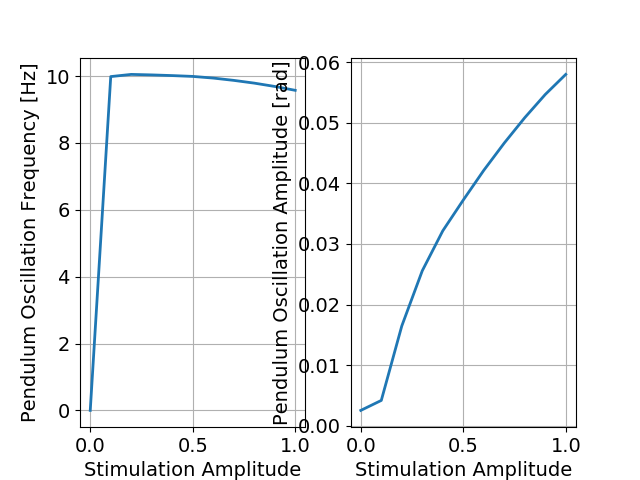
\includegraphics[width=1\textwidth]{2c_amplitude.png}

\caption{Varying Stimulation amplitude: pendulum frequency as a function of stimulation amplitude (left) and pendulum amplitude as a function of  stimulation amplitude (right)}
\label{fig:varying_amplitude}
\end{figure}
\newpage 
\begin{figure}[!h]
\centering
\includegraphics[width=1\textwidth]{2c_frequency.png} 

\caption{Varying Stimulation frequency: pendulum frequency as a function of stimulation frequency (left) and pendulum amplitude as a function of  stimulation frequency (right)}
\label{fig:varying_frequency}
\end{figure}  

\newpage
\section*{Exercise 3 : Neural network driven pendulum model with
  muscles}
\label{sec:neur-netw-driv}

\subsection*{3a. Find a set of weights for the neural network that
  produces oscillations to drive the pendulum into a limit cycle
  behavior. Plot the output of the network and the phase plot of
the pendulum}
\label{sec:4a}

We recall the 1995 Beer paper seen in class which we utilized to create 2-neuron oscillators, this is extended in the course notes to a 4 neuron oscillator. The inhibitory connections between neurons need to have negative weights, whilst the excitatory connections need to have positive weights these connections are visible on Figure \ref{fig:NNmuscle}.

\begin{figure}[!h]
\centering
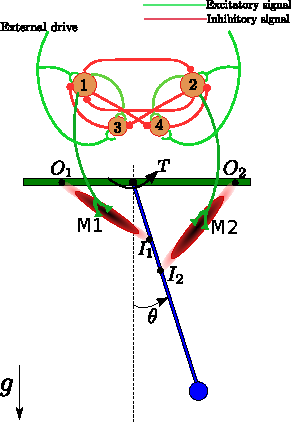
\includegraphics[width=0.31\textwidth]{Week_1/pendulum_muscles_neurons.pdf}

\caption{Muscle system with neural network showing inhibitory and excitatory connections.}
\label{fig:NNmuscle}
\end{figure}

\noindent We choose the weights given in the below matrix:
\[\begin{bmatrix}
 0   & -5 & -5 & 0 \\
-5  & 0 & 0 & -5 \\
 5  & -5 & 0 & 0 \\
-5  & 5 & 0 & 0
\end{bmatrix}\]

The membrane potential of the different neurons is given in Figure \ref{fig:neurons}. We consider the activation function to be represented by \(x = \frac{1}{1+e^(m*D)}\), the result for this is given on Figure \ref{fig:act}. 

We can clearly see the slower neurons and the faster neurons creating the oscillatory behaviour. We further notice that the output of neurons 1 and 2 controlling the muscles follow a sinusoidal pattern similar to the "artificial" activation function we applied to the system in Exercise 2. 

The Phase plot of the pendulum is given in Figure \ref{fig:phase_NN} where we can observe again a limit cycle. We did not show a perturbation here but could do so to illustrate the limit cycle behaviour. The angular position of the pendulum is also given as a function of time in Figure \ref{fig:time_NN}.
\newpage
\begin{figure}[!h]
\centering
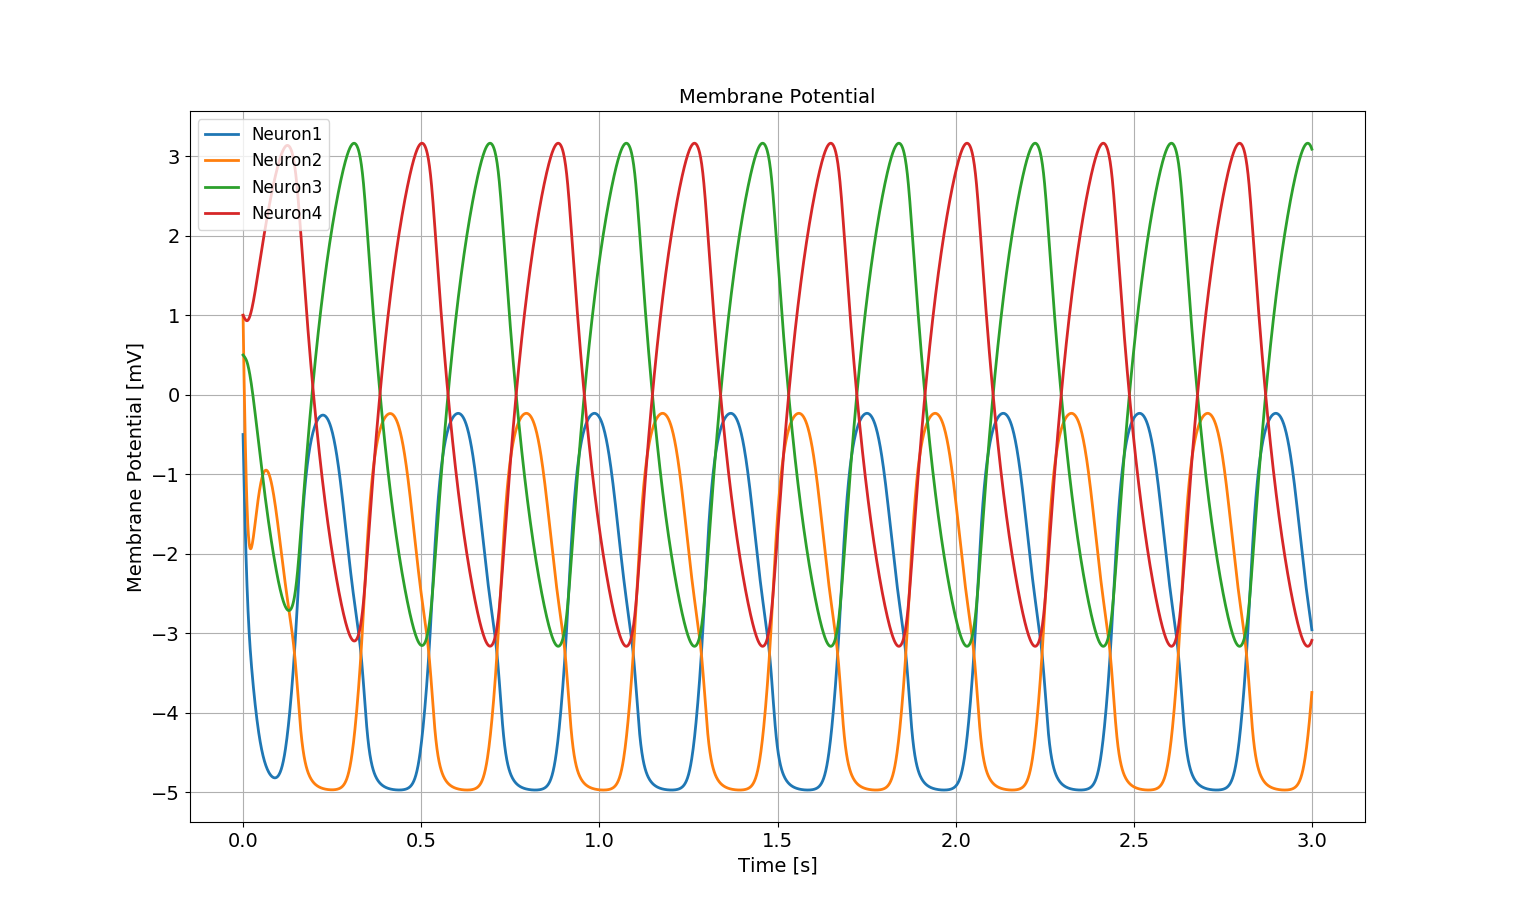
\includegraphics[width=0.8\textwidth]{membrane.png}

\caption{Response of the neural network. Membrane potentials for all 4 neurons. Neurons 1 and 2 provide the muscle activation functions.}
\label{fig:neurons}
\end{figure}

\begin{figure}[!h]
\centering
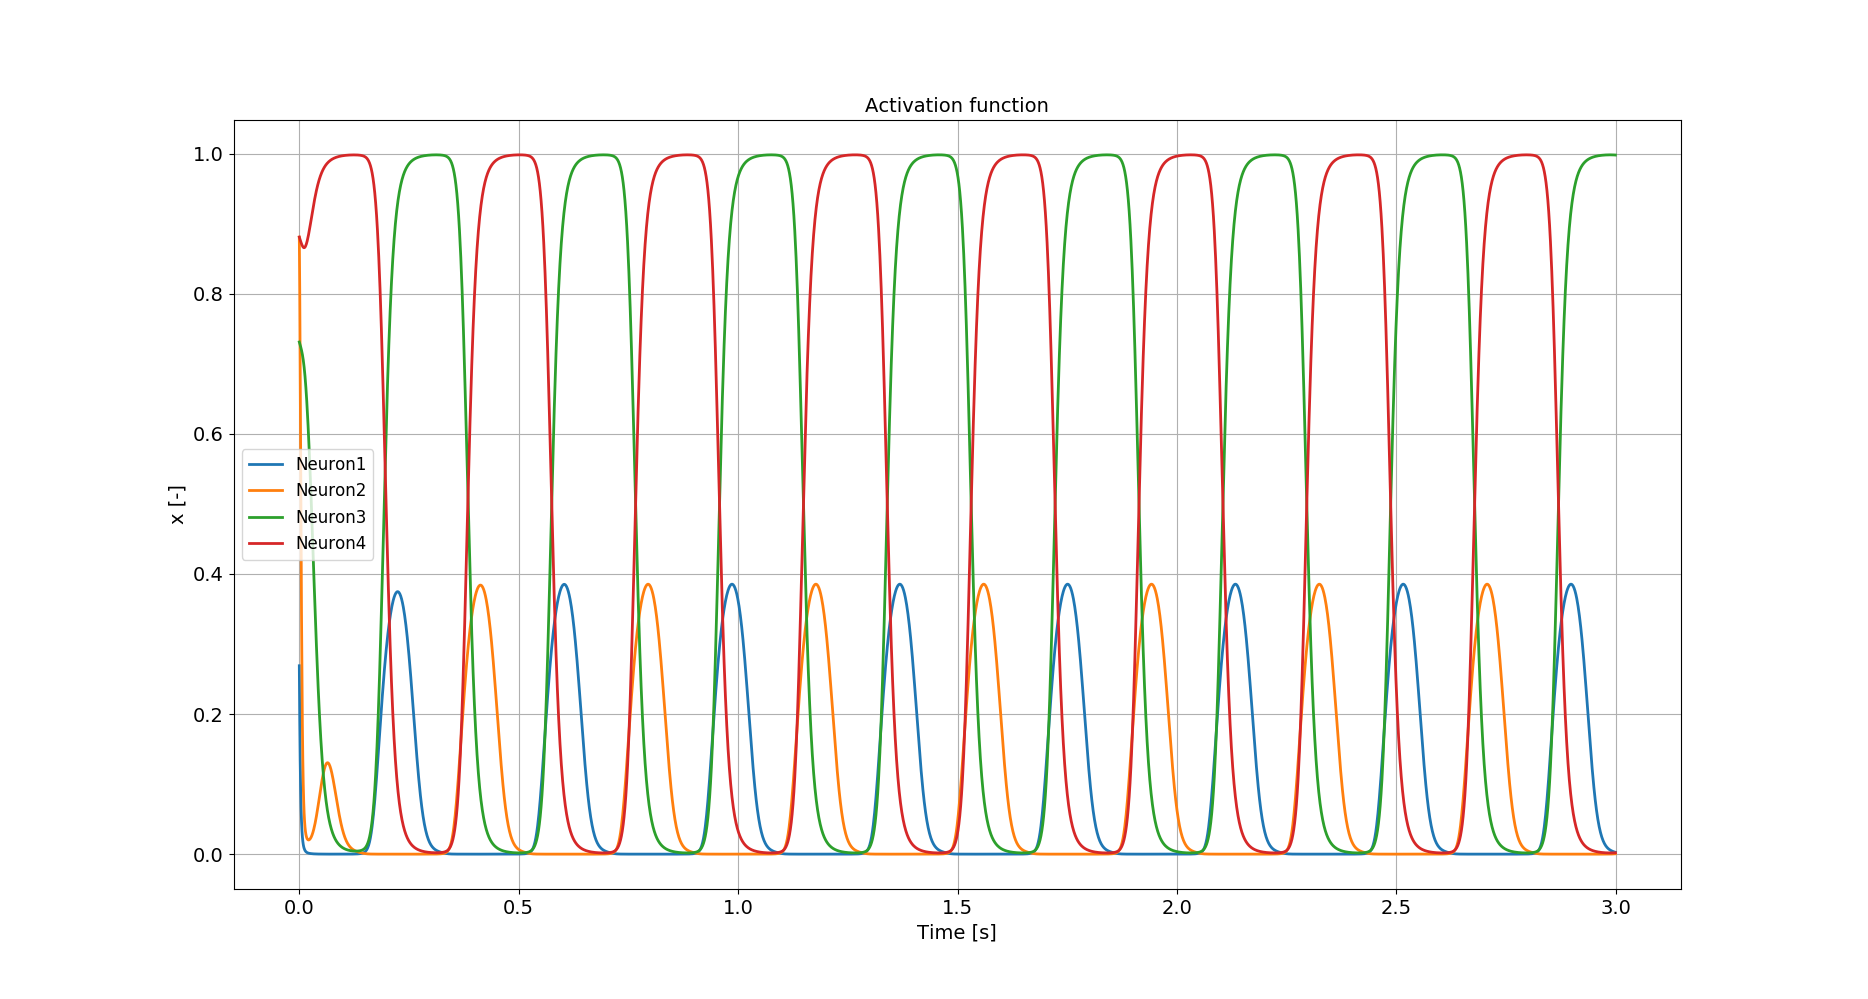
\includegraphics[width=0.8\textwidth]{act.png}

\caption{Activation function of all 4 Neurons x. The activation function of Neurons 1 and 2 drive the muscles.}
\label{fig:act}
\end{figure}

\begin{figure}[!h]
\centering
\minipage{0.49\textwidth}
\includegraphics[width=0.9\textwidth]{3a_phase.png}

\caption{Phase plot of the neural network \\ driven pendulum}
\label{fig:phase_NN}
\endminipage
\minipage{0.48\textwidth}
\centering
\includegraphics[width=1\textwidth]{3a_signal_time.png}

\caption{Neural network driven pendulum angular position }
\label{fig:time_NN}
\endminipage
\end{figure}
\newpage
\subsection*{3b. As seen in the course, apply an external drive to the
  individual neurons and explain how the system is affected. Show
  plots for low [0] and high [1] external drives. To add external
  drive to the network you can use the method \\
  \fileref{system\_simulation.py::add\_external\_inputs\_to\_network} }
\label{sec:4c}

We add the external drives using the provided function and plot the resulting pendulum phase plots on Figure \ref{fig:newphase}, the membrane potential on Figure \ref{fig:membexc} and the neuron activation functions on Figure \ref{fig:actexc}.
We notice that the muscle activation functions have a larger mean and a slightly higher frequency when the external excitation is increased. Interestingly the limit cycles of the neuron activated system are more uniform than those activated by a "perfect" sine function. Perhaps the neurons, in producing a less perfect cyclic function, start to take into account the non-linearities of the muscle system. 



\begin{figure}[!h]
\centering
\includegraphics[width=1\textwidth]{3b.png}

\caption{Phase plots of the neural network driven pendulum after adding low and high external drives }
\label{fig:newphase}
\end{figure}


\begin{figure}[!h]
\centering
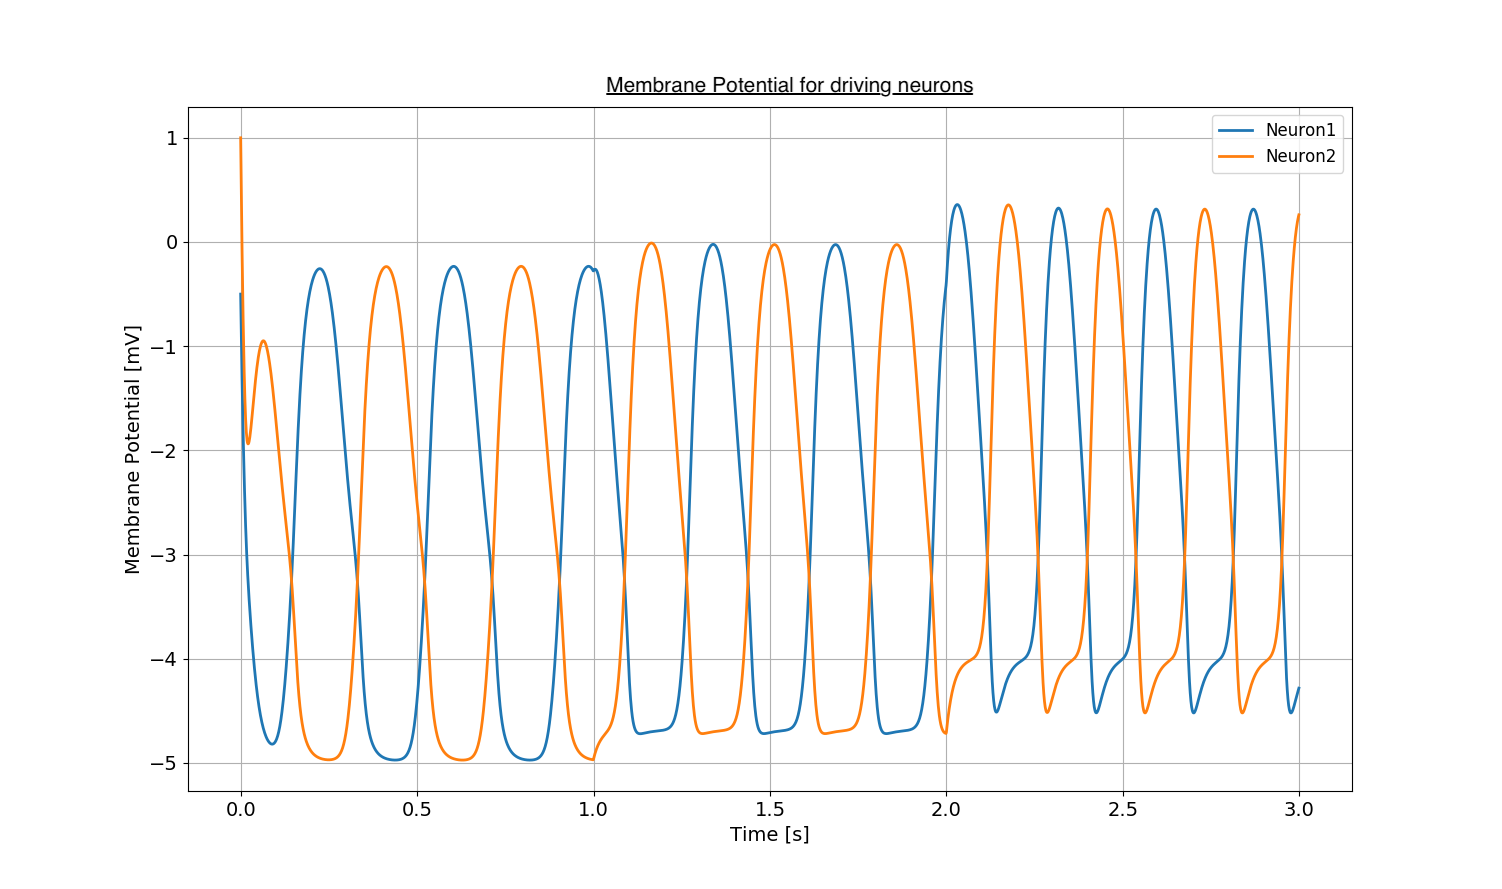
\includegraphics[width=0.7\textwidth]{mn1n2exc.png}

\caption{Membrane potential of the first two neurons driving the muscles.}
\label{fig:membexc}
\end{figure}

\begin{figure}[!h]
\centering
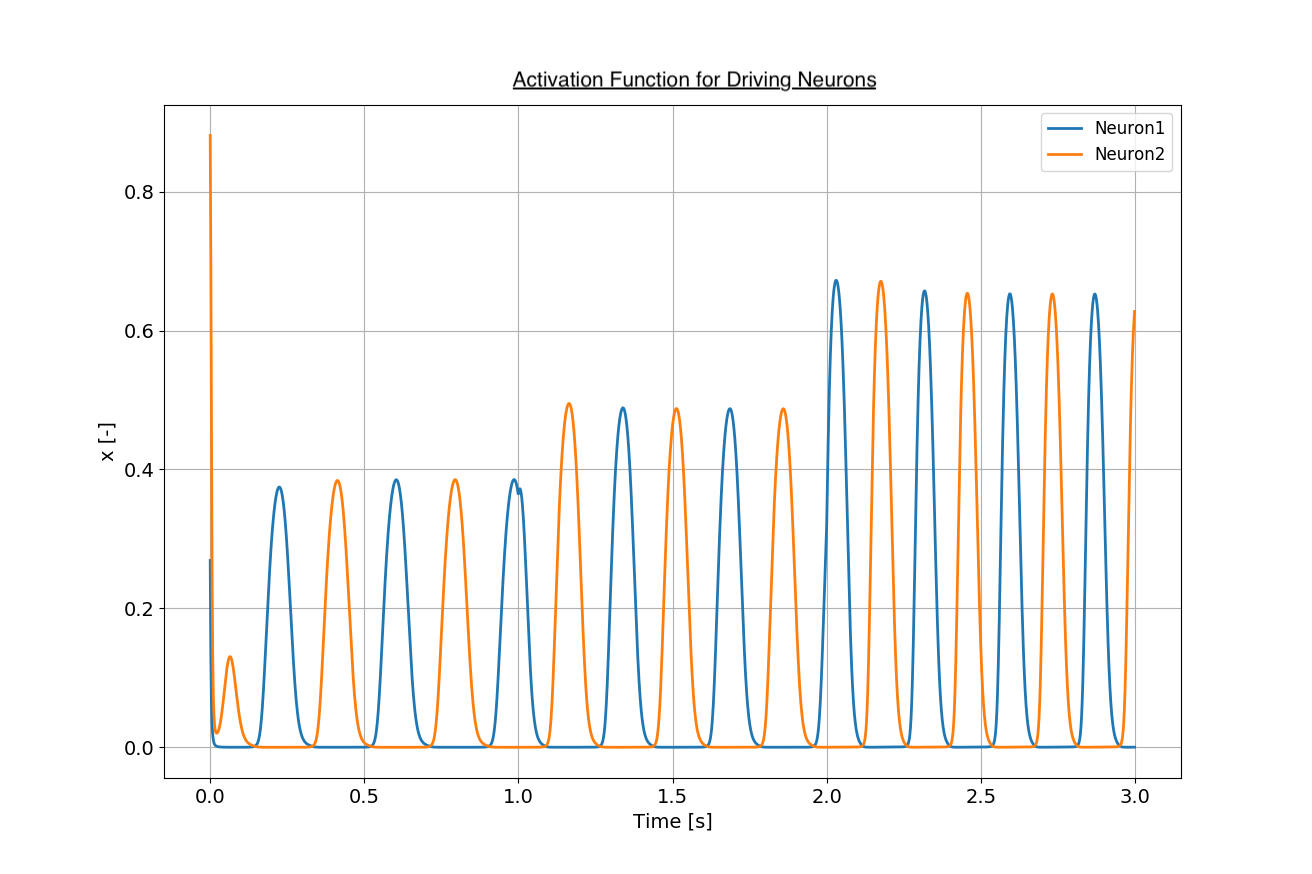
\includegraphics[width=0.7\textwidth]{xn1n2exc.png}

\caption{Activation function x of the first two neurons driving the muscles:No external drive then small external drive after t=1s and finally high external drive after t=2s}
\label{fig:actexc}
\end{figure}
\newpage 

\subsection*{3c. [Open Question] What are the limitations of the half
  center model in producing alternating patterns to control the
  pendulum? What would be the effect of sensory feedback on this
  model? (No plots required)}
\label{sec:4d}

The half center model is a very simple model that is able to produce oscillations, in this sense it might suffice to describe the simple oscillatory movement of a pendulum or a leg. In reality muscles are able to produce more complex movements, such as accelerating to a specific point and then holding at that point. This type of movement is inherently dependant on sensory feedback, requiring the eyes to return a position of the limb. Sensory feedback can also be useful for simple oscillatory movement, perhaps being able to adjust the oscillations to be in sync with other movement. A key example of this is the movement of two people together, i.e. carrying a heavy object. With sensory feedback, we can modify the gait of our model, in order to be energy efficient. For instance, a feedback on the velocity can help the CPG to make the muscle work at the appropriated gait (trot or gallop).  
\end{document}

%%% Local Variables:
%%% mode: latex
%%% TeX-master: t
%%% End: